\section{Theory}\label{Theory} 
\subsection{Nonlocality}
\begin{equation}
    p(a,b\vert x,y) = \int d\lambda \mu(\lambda) p(a\vert x,\lambda) p(b\vert y,\lambda)
\end{equation}
\begin{equation}
    S_{CHSH} = \langle A_0 B_0 \rangle + \langle A_0 B_1 \rangle + \langle A_1 B_0 \rangle -   \langle A_1 B_1 \rangle \leq 2
\end{equation}
with 
\begin{equation}
     \langle A_x B_y \rangle =  \sum_{a,b} (-1)^{a+b}p(a,b \vert x,y) 
\end{equation}
This can be violated since with 
\begin{equation}
    \begin{split}
        A_0& = \sigma_z , A_1 = \sigma_x\\
    B_0& = \frac{\sigma_x + \sigma_z}{\sqrt{2}},B_1 = \frac{\sigma_x - \sigma_z}{\sqrt{2}}
    \end{split}
\end{equation}
Leading to 
\begin{equation}
    S_{CHSH} = 2\sqrt{2} \geq 2
\end{equation}

\subsection{quantum networks}
Now we have not just one source but multiple as shown in figure \ref{fig:quantumNetwork}
\begin{figure}
    \centering
    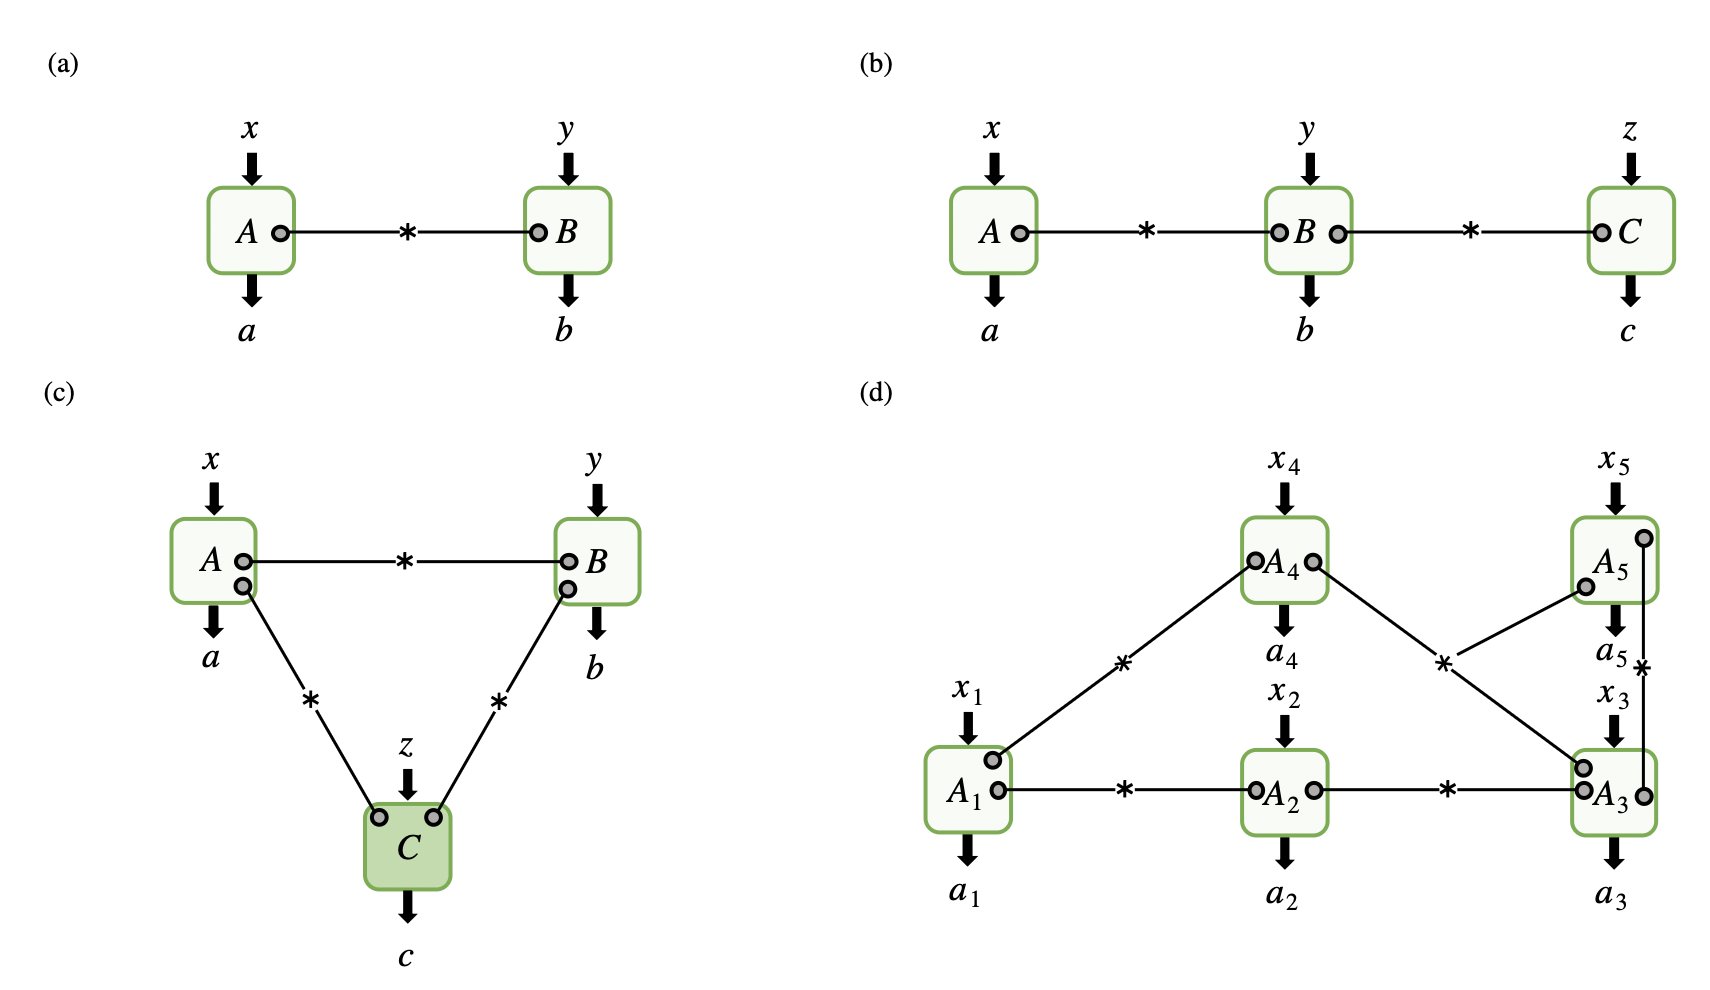
\includegraphics[width=0.8\linewidth]{Project_Quantum_Network_Nonlocality/Billeder/Quantum_Networks.png}
    \caption{(a) the common CHSH example, (b) bilocal quantum network (c) The triangle network (d) A complex network \cite{network}}
    \label{fig:quantumNetwork}
\end{figure}
This means the the bell inequality changes and is now not as simply any more.
\begin{figure}
    \centering
    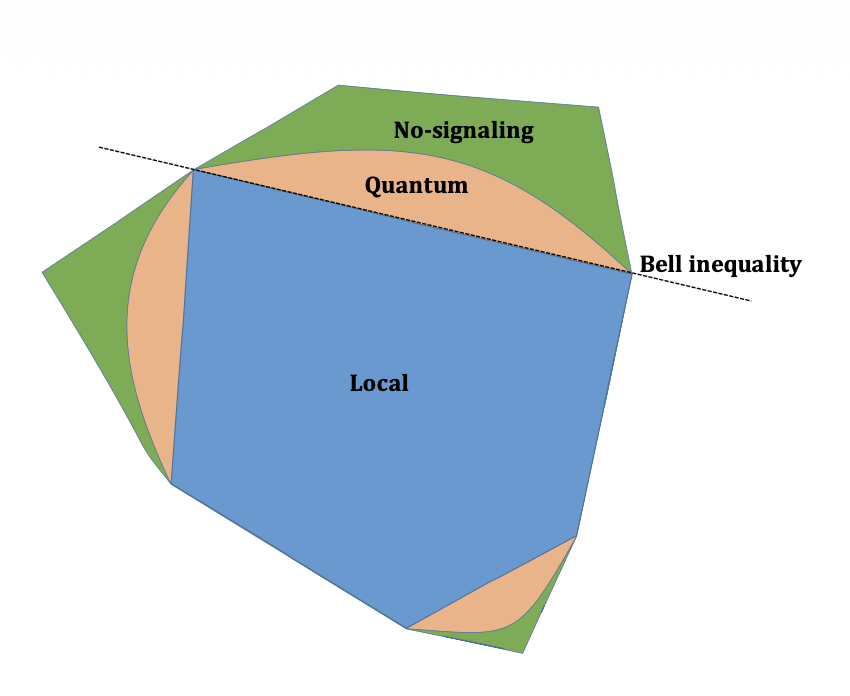
\includegraphics[width=0.8\linewidth]{Project_Quantum_Network_Nonlocality/Billeder/ploytop_CHSH.png}
    \caption{Caption}
    \label{fig:polytope_CHSH}
\end{figure}
\begin{figure}
    \centering
    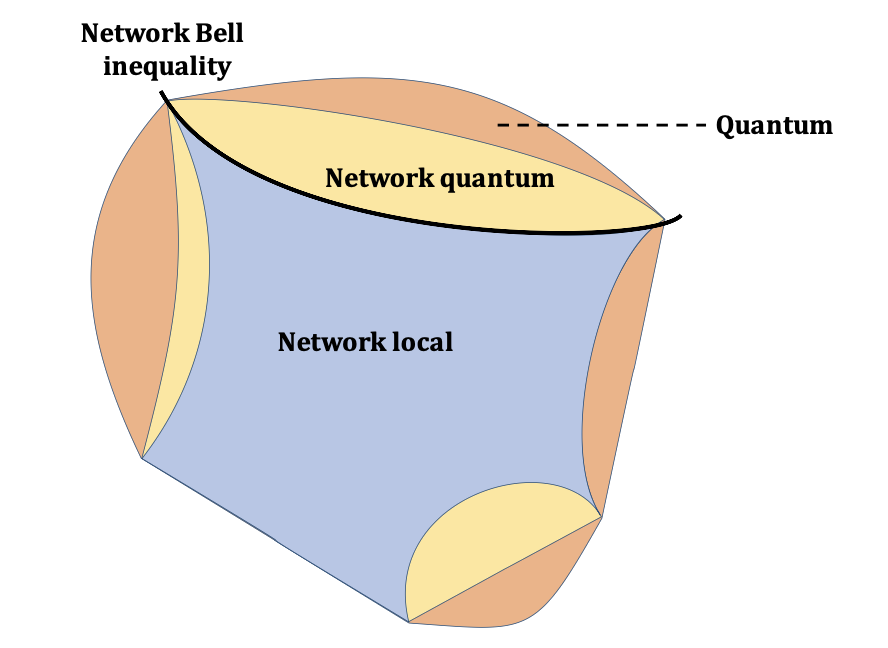
\includegraphics[width=0.8\linewidth]{Project_Quantum_Network_Nonlocality/Billeder/Polytop_Network.png}
    \caption{Caption}
    \label{fig:polytope_network}
\end{figure}
If we look at the polytope for quantum networks then we meet a problem because now the polytope is no longer convex as seen in figure \ref{fig:polytope_network} compared to \ref{fig:polytope_CHSH} 
now one can generally write that
\begin{equation}
    p(\hat{a}\vert \hat{x}) = \Trace{\left(A_{a_1 \vert x_1}^{(1)} \otimes \ldots \otimes A_{a_n \vert x_n}^{(n)} \right)\left(\rho_1 \otimes \ldots \otimes \rho_m \right)}
\end{equation}
\subsection{two examples}
Now we will go though two examples 
\subsection{triangle}
We can now write the locality expression as 
\begin{equation}
    p(a,b,c \vert x,y,z) = \int d\lambda_1 \mu_1(\lambda_1) \int d\lambda_2 \mu_2(\lambda_2) \int d\lambda_3 \mu_3(\lambda_3) \times p(a \vert x, \lambda_1, \lambda_2)p(b \vert y, \lambda_2, \lambda_3)p(c \vert z, \lambda_1, \lambda_3)
\end{equation}
